%% LyX 2.5.1 created this file.  For more info, see https://www.lyx.org/.
%% Do not edit unless you really know what you are doing.
\documentclass[journal,article,submit,pdftex,moreauthors]{Definitions/mdpi}
\usepackage{textcomp}
\usepackage[utf8]{inputenc}
\synctex=-1
\usepackage[table]{xcolor}
\usepackage{colortbl}
\usepackage{float}
\usepackage{url}
\usepackage{varwidth}
\usepackage{graphicx}

\makeatletter

%%%%%%%%%%%%%%%%%%%%%%%%%%%%%% LyX specific LaTeX commands.

\Title{Predicting Football Match Outcomes Using Machine Learning }

\Author{Morfis Sallis$^{1}$, Georgios Georgoulas$^{2}$ and Ioannis G. Tsoulos$^{3,*}$}


\address{$^{1}$\quad{}Department of Informatics and Telecommunications,
University of Ioannina, 45500 Ioannina, Greece;e.sallis@uoi.gr\\
$^{2}$\quad{}Department of Mechanical Engineering and Aeronautics,
University of Patras, Panepistimioupoli Patron, Rio 26504, Greece;
georgoul@gmail.com\\
$^{3}\quad$Department of Informatics and Telecommunications, University
of Ioannina, 45500 Ioannina, Greece; itsoulos@uoi.gr}


\corres{Correspondence: itsoulos@uoi.gr}


\abstract{Football match outcomes are influenced by a complex interplay of
dynamic team strategies and stochastic match events, posing a significant
challenge for predictive analytics. In this paper, we propose a unified
benchmarking and calibration framework for football forecasting, utilizing
a dataset of approximately 230,000 matches. We systematically compare
diverse learning paradigms---ranging from linear models (Logistic
Regression) and generalized additive frameworks (GAM) to tree structures
(FastTree, LightGBM, Random Forest) and Neural Network models (MLP).
To support future probability calibration, bookmaker odds are transformed
using the Newton--Raphson method to remove bookmaker margins. The
resulting predictive framework establishes the basis for the subsequent
integration of an Isotonic Calibration layer for probability estimation
and betting signal generation. Our empirical results demonstrate that
while methods like Random Forest excel in overall Precision (reaching
65.11\% for Home Win and 69.07\% for Away Win), the Multi-Layer Perceptron
(MLP) yields superior non-linear feature interaction mapping, achieving
the highest Recall across both markets (63.94\% and 60.25\% respectively).
Our findings show that advanced feature engineering combined with
systematic benchmarking enables the development of reliable predictive
models, while establishing the foundation for subsequent probability
calibration and betting-oriented decision support.}


\keyword{Machine learning; neural networks; stochastic techniques.}

\DeclareTextSymbolDefault{\textquotedbl}{T1}
%% Because html converters don't know tabularnewline
\providecommand{\tabularnewline}{\\}
%% Variable width box for table cells
\newenvironment{cellvarwidth}[1][t]
    {\begin{varwidth}[#1]{\linewidth}}
    {\@finalstrut\@arstrutbox\end{varwidth}}

%%%%%%%%%%%%%%%%%%%%%%%%%%%%%% User specified LaTeX commands.
%  LaTeX support: latex@mdpi.com
%  For support, please attach all files needed for compiling as well as the log file, and specify your operating system, LaTeX version, and LaTeX editor.
%=================================================================
%\documentclass[preprints,article,submit,pdftex,moreauthors]{Definitions/mdpi}
% For posting an early version of this manuscript as a preprint, you may use "preprints" as the journal. Changing "submit" to "accept" before posting will remove line numbers.
% Below journals will use APA reference format:
% admsci, aieduc, behavsci, businesses, econometrics, economies, education, ejihpe, famsci, games, humans, ijcs, ijfs, jintelligence, journalmedia, jrfm, jsam, languages, peacestud, psycholint, publications, tourismhosp, youth
% Below journals will use Chicago reference format:
% arts, genealogy, histories, humanities, laws, literature, religions, risks, socsci
%--------------------
% Class Options:
%--------------------
%----------
% journal
%----------
% Choose between the following MDPI journals:
% accountaudit, acoustics, actuators, addictions, adhesives, admsci, adolescents, aerobiology, aerospace, agriculture, agriengineering, agrochemicals, agronomy, ai, aichem, aieduc, aieng, aimater, aimed, aipa, air, aisens, algorithms, allergies, alloys, amh, analog, analytica, analytics, anatomia, anesthres, animals, antibiotics, antibodies, antioxidants, applbiosci, appliedchem, appliedmath, appliedphys, applmech, applmicrobiol, applnano, applsci, aquacj, architecture, arm, arthropoda, arts, asc, asi, astronautics, astronomy, atmosphere, atoms, audiolres, automation, axioms, bacteria, batteries, bdcc, behavsci, beverages, biochem, bioengineering, biologics, biology, biomass, biomechanics, biomed, biomedicines, biomedinformatics, biomimetics, biomolecules, biophysica, bioresourbioprod, biosensors, biosphere, biotech, birds, blockchains, bloods, blsf, brainsci, breath, buildings, businesses, cancers, carbon, cardio, cardiogenetics, cardiovascmed, catalysts, cells, ceramics, challenges, chemengineering, chemistry, chemosensors, chemproc, children, chips, cimb, civileng, cleantechnol, climate, clinbioenerg, clinpract, clockssleep, cmd, cmtr, coasts, coatings, colloids, colorants, commodities, complexities, complications, compounds, computation, computers, condensedmatter, conservation, constrmater, cosmetics, covid, crops, cryo, cryptography, crystals, csmf, ctn, culture, curroncol, cyber, dairy, data, ddc, dentistry, dermato, dermatopathology, designs, devices, dhi, diabetology, diagnostics, dietetics, digital, disabilities, diseases, diversity, dna, drones, dynamics, earth, ebj, ecm, ecologies, econometrics, economies, edm, education, eesp, ejihpe, electricity, electrochem, electronicmat, electronics, encyclopedia, endocrines, energies, eng, engproc, entomology, entropy, environments, environremediat, epidemiologia, epigenomes, esa, est, famsci, fermentation, fibers, fintech, fire, fishes, fluids, foods, forecasting, forensicsci, forests, fossstud, foundations, fractalfract, fuels, future, futureinternet, futurepharmacol, futurephys, futuretransp, galaxies, games, gases, gastroent, gastrointestdisord, gastronomy, gels, genealogy, genes, geographies, geohazards, geomatics, geometry, geosciences, geotechnics, geriatrics, germs, glacies, grasses, green, greenhealth, gucdd, hardware, hazardousmatters, healthcare, hearts, hemato, hematolrep, hep, heritage, higheredu, highthroughput, histories, horticulturae, hospitals, humanities, humans, hydrobiology, hydrogen, hydrology, hydropower, hygiene, idr, iic, ijcs, ijem, ijerph, ijfs, ijgi, ijmd, ijms, ijns, ijom, ijpb, ijt, ijtm, ijtpp, ime, immuno, informatics, information, infrastructures, inorganics, insects, instruments, inventions, iot, j, jaestheticmed, jal, jcdd, jcm, jcp, jcrm, jcs, jcto, jdad, jdb, jdream, jemr, jeta, jfb, jfmk, jgbg, jgg, jimaging, jintelligence, jlpea, jmahp, jmmp, jmms, jmp, jmse, jne, jnt, jof, joi, joitmc, joma, jop, joptm, jor, journalmedia, jox, jpbi, jphytomed, jpm, jrfm, jsam, jsan, jtaer, jvd, jzbg, kidneydial, kinasesphosphatases, knowledge, labmed, laboratories, lae, land, languages, laws, life, lights, limnolrev, lipidology, liquids, literature, livers, logics, logistics, lubricants, lymphatics, machines, macromol, magnetism, magnetochemistry, make, marinedrugs, materials, materproc, mathematics, mca, measurements, medicina, medicines, medsci, membranes, merits, metabolites, metals, meteorology, methane, metrics, metrology, micro, microarrays, microbiolres, microelectronics, micromachines, microorganisms, microplastics, microwave, minerals, mining, mmphys, modelling, molbank, molecules, mps, msf, mti, multimedia, muscles, nanoenergyadv, nanomanufacturing, nanomaterials, ncrna, ndt, network, neuroglia, neuroimaging, neurolint, neurosci, nitrogen, notspecified, nursrep, nutraceuticals, nutrients, obesities, occuphealth, oceans, ohbm, onco, optics, oral, organics, organoids, osteology, oxygen, pandemics, parasites, parasitologia, particles, pathogens, pathophysiology, peacestud, pediatrrep, pets, pharmaceuticals, pharmaceutics, pharmacoepidemiology, pharmacy, philosophies, photochem, photonics, phycology, physchem, physics, physiologia, plants, plasma, platforms, pollutants, polymers, polysaccharides, populations, poultry, powders, precipitation, precisoncol, preprints, proceedings, processes, prosthesis, proteomes, psf, psychiatryint, psychoactives, psycholint, publications, purification, quantumrep, quaternary, qubs, radiation, rdt, reactions, realestate, receptors, recycling, regeneration, religions, remotesensing, reports, reprodmed, resources, rheumato, risks, rjpm, robotics, rsee, ruminants, safety, sci, scipharm, sclerosis, seeds, sensors, separations, sexes, shi, signals, sinusitis, siuj, skins, smartcities, sna, societies, socsci, software, soilsystems, solar, solids, spectroscj, sports, standards, stats, std, stratsediment, stresses, surfaces, surgeries, suschem, sustainability, symmetry, synbio, systems, tae, targets, taxonomy, technologies, telecom, test, textiles, thalassrep, therapeutics, thermo, timespace, tomography, tourismhosp, toxics, toxins, tph, transplantology, transportation, traumacare, traumas, tri, tropicalmed, universe, urbansci, uro, vaccines, vehicles, venereology, vetsci, vibration, virtualworlds, viruses, vision, waste, water, welding, wem, wevj, wild, wind, women, world, youth, zoonoticdis
%---------
% article
%---------
% The default type of manuscript is "article", but can be replaced by:
% abstract, addendum, article, book, bookreview, briefreport, casereport, comment, commentary, communication, conferenceproceedings, correction, conferencereport, entry, expressionofconcern, extendedabstract, datadescriptor, editorial, essay, erratum, hypothesis, interestingimage, obituary, opinion, projectreport, reply, retraction, review, perspective, protocol, shortnote, studyprotocol, systematicreview, supfile, technicalnote, viewpoint, guidelines, registeredreport, tutorial
% supfile = supplementary materials
%----------
% submit
%----------
% The class option "submit" will be changed to "accept" by the Editorial Office when the paper is accepted. This will only make changes to the frontpage (e.g., the logo of the journal will get visible), the headings, and the copyright information. Also, line numbering will be removed. Journal info and pagination for accepted papers will also be assigned by the Editorial Office.
%------------------
% moreauthors
%------------------
% If there is only one author the class option oneauthor should be used. Otherwise use the class option moreauthors.
%---------
% pdftex
%---------
% The option pdftex is for use with pdfLaTeX. If eps figures are used, remove the option pdftex and use LaTeX and dvi2pdf.
%=================================================================
% MDPI internal commands - do not modify
\firstpage{1}
\setcounter{page}{\@firstpage}
\pubvolume{1}
\issuenum{1}
\articlenumber{0}
\pubyear{2026}
\copyrightyear{2026}
%\externaleditor{Firstname Lastname} % More than 1 editor, please add `` and '' before the last editor name
\datereceived{}
\daterevised{ } % Comment out if no revised date
\dateaccepted{}
\datepublished{}
%\datecorrected{} % For corrected papers include a "Corrected: XXX" date in the original paper.
%\dateretracted{} % For retracted papers include a "RETRACTED: XXX" date in the original paper.
%\doinum{} % Used for some special journals, like molbank
%\pdfoutput=1 % Uncommented for upload to arXiv.org
%\CorrStatement{yes}  % For updates
%\longauthorlist{yes} % For many authors that exceed the left citation part
%\IsAssociation{yes} % For association journals
%=================================================================
% Add packages and commands here. The following packages are loaded in our class file: fontenc, inputenc, calc, indentfirst, fancyhdr, graphicx, epstopdf, lastpage, ifthen, lineno, float, amsmath, setspace, enumitem, mathpazo, booktabs, titlesec, etoolbox, tabto, xcolor, soul, multirow, microtype, tikz, totcount, changepage, attrib, upgreek, cleveref, amsthm, hyphenat, natbib, hyperref, footmisc, url, geometry, newfloat, caption
%=================================================================
%% Please use the following mathematics environments: Theorem, Lemma, Corollary, Proposition, Characterization, Property, Problem, Example, ExamplesandDefinitions, Hypothesis, Remark, Definition, Notation, Assumption
%% For proofs, please use the proof environment (the amsthm package is loaded by the MDPI class).
%=================================================================
% The fields PACS, MSC, and JEL may be left empty or commented out if not applicable
%\PACS{J0101}
%\MSC{}
%\JEL{}
%%%%%%%%%%%%%%%%%%%%%%%%%%%%%%%%%%%%%%%%%%
% Only for the journal Diversity
%\LSID{\url{http://}}
%%%%%%%%%%%%%%%%%%%%%%%%%%%%%%%%%%%%%%%%%%
% Only for the journal Applied Sciences:
%\featuredapplication{Authors are encouraged to provide a concise description of the specific application or a potential application of the work. This section is not mandatory.}
%%%%%%%%%%%%%%%%%%%%%%%%%%%%%%%%%%%%%%%%%%
%%%%%%%%%%%%%%%%%%%%%%%%%%%%%%%%%%%%%%%%%%
% Only for the journal Data:
%\dataset{DOI number or link to the deposited data set in cases where the data set is published or set to be published separately. If the data set is submitted and will be published as a supplement to this paper in the journal Data, this field will be filled by the editors of the journal. In this case, please make sure to submit the data set as a supplement when entering your manuscript into our manuscript editorial system.}
%\datasetlicense{license under which the data set is made available (CC0, CC-BY, CC-BY-SA, CC-BY-NC, etc.)}
%%%%%%%%%%%%%%%%%%%%%%%%%%%%%%%%%%%%%%%%%%
% Only for the journal BioTech, Fishes, Neuroimaging and Toxins
%\keycontribution{The breakthroughs or highlights of the manuscript. Authors can write one or two sentences to describe the most important part of the paper.}
%%%%%%%%%%%%%%%%%%%%%%%%%%%%%%%%%%%%%%%%%%
% Only for the journal Encyclopedia
%\encyclopediadef{Instead of the abstract}
%\entrylink{The Link to this entry published on the encyclopedia platform.}
%%%%%%%%%%%%%%%%%%%%%%%%%%%%%%%%%%%%%%%%%%
%%%%%%%%%%%%%%%%%%%%%%%%%%%%%%%%%%%%%%%%%%
% Different journals have different requirements. Please check the specific journal guidelines in the "Instructions for Authors" on the journal's official website.
%\addhighlights{yes}
%\renewcommand{\addhighlights}{%
%
%\noindent The goal is to increase the discoverability and readability of the article via search engines and other scholars. Highlights should not be a copy of the abstract, but a simple text allowing the reader to quickly and simplified find out what the article is about and what can be cited from it. Each of these parts should be devoted up to 2 bullet points.\vspace{3pt}\\
%\textbf{What are the main findings?}
% \begin{itemize}[labelsep=2.5mm,topsep=-3pt]
% \item First bullet.
% \item Second bullet.
% \end{itemize}\vspace{3pt}
%\textbf{What are the implications of the main findings?}
% \begin{itemize}[labelsep=2.5mm,topsep=-3pt]
% \item First bullet.
% \item Second bullet.
% \end{itemize}
%}
%%%%%%%%%%%%%%%%%%%%%%%%%%%%%%%%%%%%%%%%%%

\makeatother

\begin{document}
\maketitle

\section{Introduction}

Many real world problems can be tackled by the so - called machine
learning tools. Among these problems one can find cases derived from
various scientific fields, such as physics \citep{physics_ml1,physics_ml2},
astronomy \citep{astronomy_ml1,astronomy_ml2}, chemistry \citep{chemistry_ml1,chemistry_ml2},
medicine \citep{med_ml1,med_ml2}, economics \citep{econ_ml1,econ_ml2},
image processing \citep{nn_image}, time series forecasting \citep{nn_timeseries}
etc. Common machine learning tools are artificial neural networks
\citep{nn1,nn2}, decision trees \citep{dt1,dt2}, support vector
machines (SVM) \citep{svm1,svm2} etc. In this research study, we
address the problem of predicting the outcome of a football match
by examining it through a variety of machine learning techniques.
This problem was tackled by various researches during the past years. 

Predicting football match outcomes is difficult because of the high
levels of noise, changing team strategies, and unpredictable match
events. Standard predictive models often struggle in these volatile
environments. This research is important for three main reasons: First,
it addresses the core issue of probability calibration in sports analytics.
Machine learning models often produce raw scores that do not reflect
real-world probabilities, especially when the data is noisy. By implementing
methods like Isotonic Calibration and using the Newton--Raphson \citep{power}
approach to remove bookmaker margins, we provide a framework that
transforms biased model outputs into reliable, objective probabilities.
Second, we conduct a rigorous comparative analysis under strictly
uniform conditions. Instead of focusing on just one algorithm, we
test fundamentally different models---including linear models, GAM
\citep{gam}, tree structures (FastTree \citep{fasttree}, LightGBM
\citep{lightgbm}, Random Forest \citep{randomForest}), and Neural
Network models (MLP)---using the exact same input features. This
provides an unbiased look at how each model handles the non-linearity
and volatility of sports data. Finally, from a practical standpoint,
this research highlights the important trade-off between Precision
and Recall in different betting markets. Whether we are analyzing
Home Win and Away Win markets, finding the right balance is essential.
Our results show that the Multi-Layer Perceptron (MLP), when integrated
into our calibrated framework, consistently maximizes the recovery
of hidden value (Recall) without sacrificing overall predictive accuracy.
Ultimately, this work helps bridge the gap between simple statistical
forecasting and more practical, value-driven risk management in sports
betting.

For example, Hvattum et al. proposed the incorporation of ELO ratings
for the prediction of match outcomes in their study \citep{elo_football}.
Also, Owramipur et al. suggested the usage of Baysian networks \citep{ml_bayesian}
to predict the outcomes for the Spanish League Barcelona team \citep{bayesian_football}.
Similarly, Presetio et al. proposed the incorporation of logistic
regression \citep{ml_logistic} to predict the outcomes of football
matches \citep{logistic_football}. Moreover, Martins et al. used
a polynomial classifier for the prediction of football outcomes \citep{polynomial_football}.
Schauberger et al. selected the method of random forests to predict
the results of football matches in their study \citep{rf_football}.
Various attributes of football players was studied by Danisk et al.
in order to predict the result of football matches in their related
paper \citep{attr_football}. Constantinou proposed a new machine
learning model, named Dolores which is based on Hybrid Bayesian Networks,
to predict football match outcomes from datasets selected in a series
of countries \citep{dolores_football}. Baboota et al. applied gradient
boosting \citep{ml_boosting} for English Premier League \citep{boost_football}.
Additionally, a deep learning framework was designed from Rahman to
tackle the problem of prediction football results \citep{deep_football}. 

To address the limitations of individual algorithms and the common
issue of probability distortion in sports forecasting, we propose
a unified benchmarking and calibration framework. Our methodology
focuses on three core contributions:
\begin{itemize}
\item A Consistent Feature Engineering Pipeline: We build a predictive feature
vector that combines dynamic team performance indicators---such as
Elo ratings \citep{elo_football}, Home Clean Sheet, and Away Fail-To-Score
ratios---with raw bookmaker market odds. These odds are systematically
adjusted using the Newton--Raphson method to isolate the intrinsic
probabilities and remove market margins.
\item Comprehensive Architectural Benchmarking: We conduct a comparative
evaluation of different learning paradigms under strictly uniform
conditions. By testing models ranging from linear approaches (Logistic
Regression) and generalized additive frameworks (GAM) to tree structures
(FastTree , LightGBM, Random Forest) and Neural Network models (MLP),
we provide an unbiased look at how different models handle the high-dimensional
volatility of football data.
\item Framework for Robust Betting Signals: To bridge the gap between model
scores and actionable betting decisions, we propose the integration
of an Isotonic Calibration layer as part of this framework. While
the present study focuses on establishing and benchmarking the underlying
predictive models, this calibration layer --- to be applied in the
next research phase --- is intended to transform raw output scores
into mathematically objective probabilities, enabling the derivation
of robust betting signals. As empirical results demonstrate, this
process highlights clear performance trends across both the Home Win
and Away Win markets:
\begin{itemize}
\item Performance Stability: Linear models and methods, such as Logistic
Regression and Random Forest, provide high structural stability and
consistently competitive Precision across both markets.
\item Non-Linear Interaction Mapping: The Multi-Layer Perceptron (MLP) acts
as the most balanced model, consistently achieving the highest Recall
in both markets. This suggests that the MLP is better at mapping complex
feature interactions and identifying matches with higher expected
betting value that traditional statistical models often miss.
\end{itemize}
\item Reproducible Large-Scale Evaluation: Unlike many previous studies
that evaluate a single predictive model or employ heterogeneous experimental
settings, all algorithms are trained and evaluated using the same
large-scale dataset, an identical feature space, and a chronological
train--test split that better reflects real-world forecasting conditions
while preventing information leakage. This unified evaluation protocol
enables a fair comparison of fundamentally different machine learning
paradigms and improves the reproducibility of the reported results.
\end{itemize}
Overall, the proposed framework provides a reproducible methodology
for evaluating multiple machine learning paradigms under identical
experimental conditions. The experimental results indicate that the
MLP captures complex non-linear feature interactions more effectively
than the remaining benchmarked methods, while the Random Forest exhibits
superior precision and stability. These findings support the development
of calibrated predictive systems for football match forecasting and
subsequent probability-based decision making.

Although numerous studies have reported promising results for football
match prediction, direct numerical comparison remains challenging
because different datasets, leagues, feature sets, and evaluation
protocols are typically employed. Rather than claiming a universally
superior predictive accuracy, the present work focuses on providing
a unified and reproducible benchmarking framework in which seven fundamentally
different machine learning paradigms are evaluated under identical
experimental conditions on a large-scale dataset. This allows a fair
assessment of their relative strengths while emphasizing model stability
and probability reliability through repeated experimentation and calibration.

The remaining of this article is organized as follows: in section
\ref{sec:Materials-and-Methods} the proposed datasets and the used
methodology are fully described, in section \ref{sec:Results} the
experimental results are outlined and finally in section \ref{sec:Conclusions}
a discussion is provided based on the experimental results.

\section{Materials and Methods\label{sec:Materials-and-Methods}}

\subsection{The Dataset Employed}

In this study, we utilized a large-scale dataset of historical football
matches sourced from a professional sports analytics repository. The
data collection process prioritized high granularity, incorporating
not only match results but also advanced performance indicators and
pre-match market probabilities. The dataset's reliability is ensured
through its internal consistency and widespread use in sports forecasting
benchmarks.

\subsection{Dataset Description}

The experimental dataset comprises 225,474 match events spanning from
2018 to 2025. To ensure rigorous evaluation, the data was partitioned
into a training set of 149,998 matches and a dedicated test set of
75,476 matches. The core variables included in the raw data are summarized
in Table \ref{tab:Description-of-the}. The inclusion of \textit{LeagueId}
and \textit{SeasonPhase} allows the model to account for competitive
context and seasonal variations. To avoid information leakage and
better reflect a real-world deployment scenario, the dataset was partitioned
chronologically, with earlier seasons used for training and later
matches reserved exclusively for testing.

\begin{table}[H]
\begin{centering}
\caption{Description of the original dataset features.\label{tab:Description-of-the}}
\par\end{centering}
\centering{}%
\begin{tabular}{|ll|}
\hline 
\textbf{Feature} & \textbf{Description / Range}\tabularnewline
\hline 
\hline 
MatchDate & Temporal identifier (2018--2025)\tabularnewline
League / LeagueId & Categorical identifiers for competitive tiers\tabularnewline
HomeTeam / AwayTeam & Competing squad identifiers\tabularnewline
Label & Primary outcome target (1, X, 2)\tabularnewline
EloDiff & Difference in Elo ratings ($-500$ to $+500$)\tabularnewline
ProbHome/Draw/Away & Pre-match market probabilities (0 to 1)\tabularnewline
RankDifference & Difference in league table standings\tabularnewline
SeasonPhase & Categorical marker for season stage\tabularnewline
AttackVsDefense / DefenseVsAttack & Derived offensive and defensive interaction ratios\tabularnewline
TotalScoringPotential & Normalized long-term scoring capacity\tabularnewline
TotalDefensiveWeakness & Normalized long-term goal concession rate\tabularnewline
HomeCleanSheetRatio & Probabilistic historical clean sheet frequency\tabularnewline
AwayFTSRatio & Away team Failed-to-Score probability\tabularnewline
\hline 
\end{tabular}
\end{table}


\subsection{Feature Engineering and Mathematical Formulation}

To capture the dynamic interaction between offensive and defensive
capacities, the raw data was transformed into formal performance metrics.
Let $AvgH_{s}$ and $AvgH_{c}$ denote the average goals scored and
conceded by the home team, and $AvgA_{s},AvgA_{c}$ the corresponding
values for the away team. A smoothing constant $\epsilon=0.01$ was
applied to prevent division by zero.
\begin{description}
\item [{AttackVsDefense:}] Represents the home team's offensive efficiency
relative to the away team's defensive record:
\begin{equation}
\mbox{AttackVsDefense}=\frac{AvgH_{s}}{AvgA_{c}+\epsilon}\label{eq:attack_vs_defense}
\end{equation}
\item [{DefenseVsAttack:}] Quantifies the home team's defensive capability
against the away team's scoring force:
\begin{equation}
\mbox{DefenseVsAttack}=\frac{AvgH_{c}}{AvgA_{s}+\epsilon}\label{eq:defensevsattack}
\end{equation}
\item [{TotalScoringPotential:}] Modeled as the numerical difference between
home and away scoring capacities, identifying the relative offensive
edge:
\begin{equation}
\mbox{TotalScoringPotential}=AvgH_{s}-AvgA_{s}\label{eq:totalscoringpotential}
\end{equation}
\item [{TotalDefensiveWeakness:}] Assesses the relative vulnerability of
the home defense compared to the away defense as a ratio:
\begin{equation}
\mbox{TotalDefensiveWeakness}=\frac{AvgH_{c}}{AvgA_{c}+\epsilon}\label{eq:totaldefensiveweakness}
\end{equation}
\item [{\textit{HomeCleanSheetRatio}}] (HCSR) and \textbf{\textit{AwayFTSRatio}}
(AFTS) capture probabilistic historical frequencies:
\begin{equation}
HCSR=\frac{\sum^{N}_{i=1}\mathbb{I}(G_{H,c}=0)}{N},\quad AFTS=\frac{\sum^{N}_{j=1}\mathbb{I}(G_{A,s}=0)}{N}\label{eq:HCSR}
\end{equation}
\end{description}

\subsection{Feature Importance Motivation}

The generated feature space is explicitly designed to satisfy three
essential, complementary operational criteria: 
\begin{enumerate}
\item Long-term structural team performance using rating systems (\textit{EloDiff},
\textit{RankDifference}). 
\item Granular tactical interaction effects (\textit{AttackVsDefense}, \textit{DefenseVsAttack}).
\item Distribution-based prior probabilities derived from betting market
evaluations (\textit{ProbHome}, \textit{ProbDraw}, \textit{ProbAway}).
This multi-source configuration mitigates model vulnerability to single-feature
bias and improves generalization accuracy.
\end{enumerate}

\section{Results\label{sec:Results}}

\subsection{Experimental settings }

For the development and training of the predictive models for sports
outcomes, the ML.NET \citep{ml.net} framework was employed---an
open-source, cross-platform machine learning framework developed by
Microsoft. The choice of ML.NET was driven by its capability to integrate
sophisticated algorithms, such as FastForest (a highly optimized implementation
of the Random Forest ), which offers both computational efficiency
and robustness when handling large-scale datasets. To evaluate the
stability of the models, a 30-run stability analysis was conducted.
This rigorous validation process ensured consistent performance metrics
(Error, Precision, and Recall) and minimized the risk of overfitting,
thereby validating the model's reliability for analyzing noisy, real-world
data. The following methods were incorporated in the conducted experiments
from ML.NET:
\begin{enumerate}
\item FastTree \citep{fasttree}.
\item Gam \citep{gam}.
\item LightGBM \citep{lightgbm}.
\item Logistic Regression \citep{ml_logistic}.
\item MLP, that denotes an artificial neural network \citep{nn1,nn2} with
10 processing nodes. This network is trained using the L-BFGS method
\citep{lbfgs}.
\item Random Forest \citep{randomForest}.
\item RBF, that denotes a Radial Basis Function network \citep{rbf1,rbf2}. 
\end{enumerate}
The MLP was trained with 10 L-BFGS iterations (Table 2). To confirm
this was sufficient for convergence, a control run with 100 iterations
was also conducted; the resulting Precision, Recall, and Error values
differed by no more than 1.1 percentage points from those reported
in Tables 3 and 4 for both markets, confirming that the model had
already converged within the original 10-iteration budget.

\vspace{6pt}

Table \ref{tab:Experimental-settings.} presents the parameters used
by the machine learning methods employed in the conducted experiments.

\begin{table}[H]
\caption{Experimental settings.\label{tab:Experimental-settings.}}

\centering{}%
\begin{tabular}{|c|c|c|}
\hline 
METHOD & PARAMETER & VALUE\tabularnewline
\hline 
\hline 
FASTTREE & Leaves & 20\tabularnewline
\hline 
FASTTREE & Trees & 600\tabularnewline
\hline 
FASTTREE & MinExample & 100\tabularnewline
\hline 
FASTTREE & LearnRate & 0.05\tabularnewline
\hline 
FASTTREE & FeatureFraction & 0.9\tabularnewline
\hline 
RandomForest & Leaves & 20\tabularnewline
\hline 
RandomForest & Trees & 100\tabularnewline
\hline 
RandomForest & MinExample & 10\tabularnewline
\hline 
RandomForest & FeatureFraction & 0.8\tabularnewline
\hline 
LightGBM & Leaves & 31\tabularnewline
\hline 
LightGBM & MinExample & 20\tabularnewline
\hline 
LightGBM & LearnRate & 0.1\tabularnewline
\hline 
LightGBM & Iterations & 100\tabularnewline
\hline 
GAM & Iterations & 100\tabularnewline
\hline 
GAM & MaxBinCount & 255\tabularnewline
\hline 
GAM & LearnRate & 0.1\tabularnewline
\hline 
RBF & Clusters (K-means) & 2\tabularnewline
\hline 
RBF & Sigma (Gaussian) & 1.4\tabularnewline
\hline 
RBF & MaxIter & 200\tabularnewline
\hline 
MLP & LBFGS Iterations & 10\tabularnewline
\hline 
\begin{cellvarwidth}[t]
\centering
Logistic \\
Regression
\end{cellvarwidth} & L2Regularization & 0.1\tabularnewline
\hline 
\begin{cellvarwidth}[t]
\centering
Logistic \\
Regression
\end{cellvarwidth} & Tolerance & $10^{-4}$\tabularnewline
\hline 
\end{tabular}
\end{table}
 These parameters are analyzed in detail below:
\begin{enumerate}
\item \textbf{Leaves}: Defines the complexity of each tree by setting the
maximum number of leaves. A higher value allows the model to capture
more complex patterns but increases the risk of overfitting.
\item \textbf{Trees}: Specifies the total number of trees to build. Increasing
this number generally improves model stability and predictive performance
but requires more training time.
\item \textbf{MinExample}:Sets the minimum number of data samples required
to create a leaf. This acts as a regularization mechanism; higher
values prevent the model from learning from noise or outliers.
\item \textbf{LearnRate}: Controls the contribution of each tree to the
final prediction. A lower learning rate makes the optimization process
more robust, requiring more trees to reach an optimal solution.
\item \textbf{FeatureFraction}: Determines the percentage of features to
consider when building each tree. Using a fraction (e.g., $0.8$)
introduces randomness, which helps the model avoid focusing too heavily
on a single feature and improves generalization.
\item \textbf{MaximumIterations} (Iterations): The number of times the algorithm
passes through the entire training dataset to update weights.
\item \textbf{MaxBinCount}: Sets the maximum number of bins used to group
features, helping to discretize continuous variables for more efficient
processing.
\item \textbf{Clusters} (K-Means): Defines the number of centroids (hidden
neurons) used to represent the input space. Each cluster captures
a local region of the data.
\item \textbf{Sigma} (Gaussian Spread): Controls the width of the radial
basis function (Gaussian kernel). It determines how far the influence
of a single neuron extends in the input space; a smaller sigma makes
neurons more sensitive to localized inputs.
\item \textbf{L2Regularization}: A penalty applied to the magnitude of the
model weights. It discourages overly large weights, which helps in
preventing overfitting and improves the model's ability to generalize
to unseen data.
\item \textbf{Tolerance}: The threshold for the optimization algorithm to
determine convergence. It dictates how small the improvements in the
loss function must be before the algorithm stops.
\end{enumerate}

\subsection{Experimental results}

Definition of the two binary problems. Before presenting the numerical
results, it is important to clarify how the target variable was constructed
for each market. The original dataset label (Label \ensuremath{\in}
\{1, X, 2\}) corresponds to the three-way outcome of a match (home
win, draw, away win). For the purposes of this analysis, the problem
was not treated as a three-class classification task, but was instead
reformulated into two separate binary classification problems, one
for each betting market:

Home Win market (Table \ref{tab:Home-win-experimental}): The positive
class corresponds to the outcome \textquotedbl 1\textquotedbl{} (home
win), while the classes \textquotedbl X\textquotedbl{} (draw) and
\textquotedbl 2\textquotedbl{} (away win) were merged into a single
negative class, \textquotedbl not Home Win.\textquotedbl{} In other
words, the model is asked to answer the question \textquotedbl will
the home team win or not,\textquotedbl{} collapsing the distinction
between a draw and an away win.

Away Win market (Table \ref{tab:Away-win-experimental}): Conversely,
the positive class corresponds to the outcome \textquotedbl 2\textquotedbl{}
(away win), while the classes \textquotedbl X\textquotedbl{} (draw)
and \textquotedbl 1\textquotedbl{} (home win) were merged into a
single negative class, \textquotedbl not Away Win.\textquotedbl{}

This approach was chosen because it directly mirrors how real-world
betting markets of the \textquotedbl Double Chance\textquotedbl{}
/ single-market type are structured (e.g., \textquotedbl 1\textquotedbl{}
versus \textquotedbl X2,\textquotedbl{} and \textquotedbl 2\textquotedbl{}
versus \textquotedbl 1X\textquotedbl ), and it allows each model
to be independently optimized for the specific market of interest,
without the constraints of a shared multi-class loss function. It
is worth noting that this merging directly affects class balance:
in the Away Win market, the positive class (\textquotedbl 2\textquotedbl )
is the minority category in most leagues, which partly explains the
systematically lower Recall values observed both in Table 4 and in
the per-league stability analysis (§3.3, Figures 1--3).

Table \ref{tab:Home-win-experimental} depicts the experimental results
using the incorporated method on the Home Win dataset. 

\begin{table}[H]
\caption{Home win experimental results.\label{tab:Home-win-experimental}}

\centering{}%
\begin{tabular}{|c|c|c|c|}
\hline 
MODEL & ERROR & PRECISION & RECALL\tabularnewline
\hline 
\hline 
FastTree & 34.63\% & 64.91\% & 63.28\%\tabularnewline
\hline 
GAM & 34.89\% & 64.82\% & 62.75\%\tabularnewline
\hline 
LightGBM & 34.91\% & 64.59\% & 63.00\%\tabularnewline
\hline 
\begin{cellvarwidth}[t]
\centering
Logistic \\
Regression
\end{cellvarwidth} & 34.51\% & 65.03\% & 63.44\%\tabularnewline
\hline 
MLP & 35.05\% & 64.21\% & 63.94\%\tabularnewline
\hline 
\begin{cellvarwidth}[t]
\centering
Random\\
Forest
\end{cellvarwidth} & 34.71\% & 65.11\% & 62.86\%\tabularnewline
\hline 
RBF & 44.31\% & 54.75\% & 54.71\%\tabularnewline
\hline 
\end{tabular}
\end{table}

Home Win results (Table \ref{tab:Home-win-experimental}). Table \ref{tab:Home-win-experimental}
summarizes the performance of the seven methods on the binary \textquotedbl Home
Win vs. merged X2\textquotedbl{} problem. Random Forest achieved the
highest Precision overall (65.11\%), with Logistic Regression close
behind (65.03\%) and also recording the lowest Error among all seven
methods (34.51\%). Together, these two methods confirm their role
as the most structurally stable, high-precision baselines for this
market. In contrast, the MLP, despite showing the highest error (35.05\%)
and the lowest Precision (64.21\%) in the group, stood out with the
highest Recall (63.94\%), indicating that the network recovers a larger
proportion of actual home-win instances, even at the cost of somewhat
lower precision on its positive predictions. RBF remained clearly
the weakest model (Error 44.31\%, Precision 54.75\%, Recall 54.71\%),
confirming its limited suitability for this task under the current
parameterization (Table \ref{tab:Experimental-settings.}).

Similarly, Table \ref{tab:Away-win-experimental} presents the experimental
results on the Away win dataset with the assistance of the the used
machine learning methods.
\begin{table}[H]
\caption{Away win experimental results.\label{tab:Away-win-experimental}}

\centering{}%
\begin{tabular}{|c|c|c|c|}
\hline 
MODEL & ERROR & PRECISION & RECALL\tabularnewline
\hline 
\hline 
FastTree & 27.97\% & 68.04\% & 59.29\%\tabularnewline
\hline 
GAM & 28.07\% & 68.64\% & 58.36\%\tabularnewline
\hline 
LightGBM & 27.96\% & 68.07\% & 59.31\%\tabularnewline
\hline 
\begin{cellvarwidth}[t]
\centering
Logistic \\
Regression
\end{cellvarwidth} & 27.82\% & 68.21\% & 59.66\%\tabularnewline
\hline 
MLP & 27.90\% & 67.59\% & 60.25\%\tabularnewline
\hline 
\begin{cellvarwidth}[t]
\centering
Random\\
Forest
\end{cellvarwidth} & 27.96\% & 69.07\% & 58.39\%\tabularnewline
\hline 
RBF & 32.62\% & 56.68\% & 52.91\%\tabularnewline
\hline 
\end{tabular}
\end{table}

Away Win results (Table \ref{tab:Away-win-experimental}). In the
binary \textquotedbl Away Win vs. merged X1\textquotedbl{} problem,
absolute error levels are lower than in the Home Win market (Error
27.82\%--28.07\% for the six strongest methods), reflecting the fact
that away wins occur less frequently overall, which mechanically lowers
the baseline error rate for a model that leans conservative. Random
Forest again delivered the highest Precision (69.07\%), followed by
GAM (68.64\%) and Logistic Regression (68.21\%), reinforcing the pattern
observed in the Home Win market: tree-based and linear methods excel
at producing high-confidence positive predictions. The MLP, once more,
achieved the highest Recall (60.25\%) while trailing slightly in Precision
(67.59\%) and Error (27.90\% --- still competitive, and in fact better
than several tree-based alternatives). RBF again underperformed substantially
across all three metrics (Error 32.62\%, Precision 56.68\%, Recall
52.91\%), confirming its consistent weakness across both markets.

Overall pattern. Taken together, Table \ref{tab:Home-win-experimental}
and Table \ref{tab:Away-win-experimental} reveal a consistent trade-off
across both merged binary formulations: Random Forest and Logistic
Regression prioritize Precision and stability, making fewer but more
confident positive predictions, whereas the MLP prioritizes Recall,
capturing a larger share of true positive outcomes (whether \textquotedbl Home
Win\textquotedbl{} or \textquotedbl Away Win\textquotedbl ) at a
modest cost in precision. This trade-off is directly relevant to betting-signal
generation, since a higher-Recall model such as the MLP is more likely
to surface value opportunities that higher-Precision models miss,
while a higher-Precision model such as Random Forest is more likely
to minimize false-positive betting signals. This distinction motivates
the subsequent stability analysis in §3.3, where the behavior of the
(higher-Precision) Random Forest model is examined in greater depth
across leagues and repeated runs, and it also motivates the planned
Isotonic Calibration layer, which aims to reconcile these Precision/Recall
trade-offs into a single, well-calibrated probability estimate for
each of the two merged binary markets.

\subsection{Statistics}

The following five figures were produced from the 30-run stability
analysis and the overall model-comparison results contained in the
accompanying experimental workbook. They are intended to supplement
the experimental results with a visual, league-level and run-level
view of model robustness, and to support the completed Conclusions
section at the end of this document. The Figure \ref{fig:meanTrees}
illustrates the average precision, recall, and classification error
achieved by the Random Forest model (200 trees, averaged over 30 runs)
for the Home Win and Away Win markets. The results are reported for
both the pooled dataset (\textquotedbl All Leagues\textquotedbl )
and each of the ten leagues evaluated individually. 

\vspace{6pt}

\begin{figure}[H]
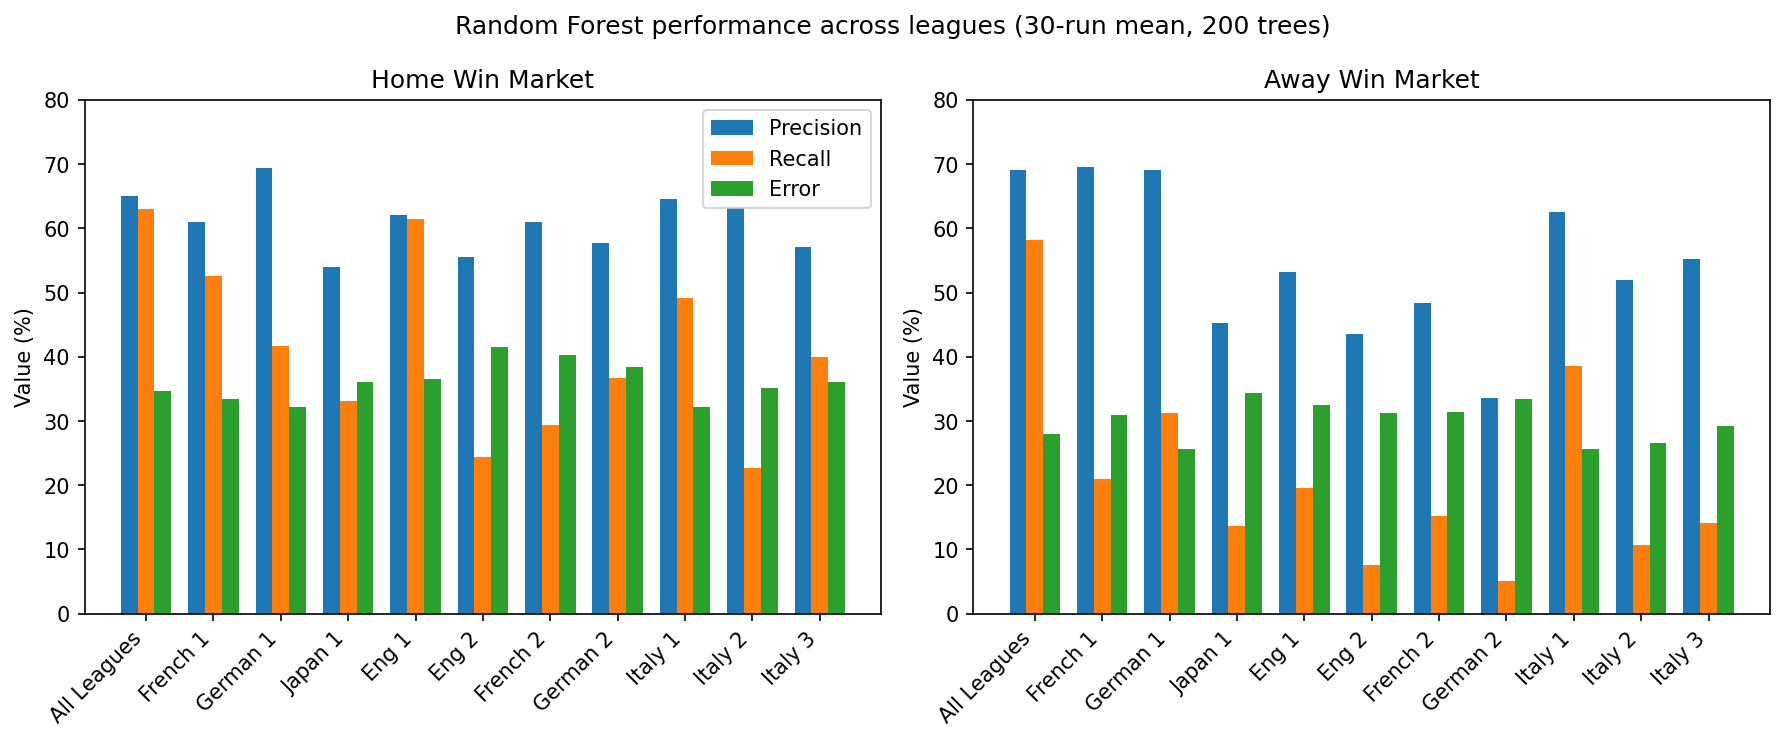
\includegraphics[scale=0.4]{all4}

\caption{Mean Precision, Recall and Error (\%) of the Random Forest model (200
trees, 30-run average) for the Home Win and Away Win markets, compared
across the pooled dataset (\textquotedbl All Leagues\textquotedbl )
and the ten individually evaluated leagues.\label{fig:meanTrees}}

\end{figure}
The grouped comparison, now extended to all ten individually evaluated
leagues alongside the pooled dataset, confirms that Precision remains
comparatively stable across leagues (53.98\% for Japan 1 to 69.36\%
for German 1, Home Win; 33.60\% for German 2 to 69.52\% for French
1, Away Win), while Recall is markedly more league-dependent. For
the Away Win market, Recall collapses from 58.24\% on the pooled dataset
to as low as 5.13\% (German 2) and 7.55\% (Eng 2), and reaches at
most 38.55\% (Italy 1) among the individually evaluated leagues ---
still well below the pooled figure. Home Win shows the same pattern,
with Recall ranging from 22.74\% (Italy 2) up to 61.49\% (Eng 1),
the latter being the only individual league to approach the pooled
model's 63.04\%. Since Away Win is already the minority outcome class
in most domestic leagues, restricting training and evaluation to a
single, smaller league sharply reduces the number of positive examples
available to the model, consistently pushing the classifier towards
more conservative, higher-precision but lower-recall behaviour.

\begin{figure}[H]
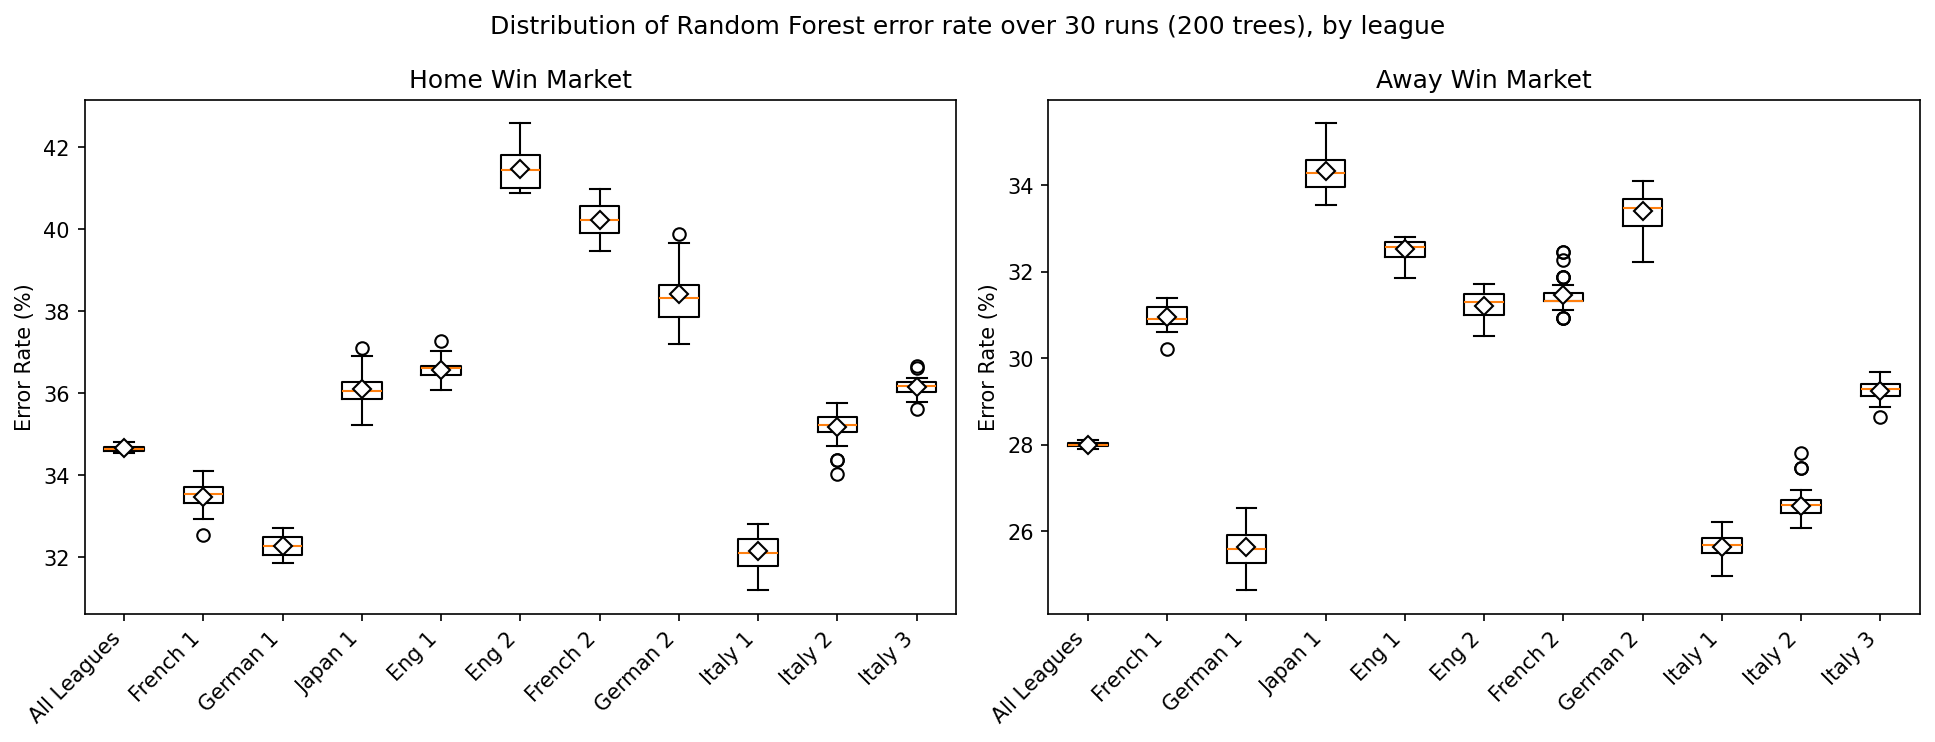
\includegraphics[scale=0.4]{all3}\caption{Distribution of the Random Forest Error Rate (\%) over 30 independent
runs (200 trees), shown separately for the Home Win and Away Win markets
and for each league subset. Diamonds mark the mean; the horizontal
line marks the median; circles denote outlier runs.\label{fig:Distribution-of-the}}
\end{figure}
\vspace{6pt}
The box plot presented in Figure \ref{fig:Distribution-of-the} is
the clearest evidence of statistical stability in the study. The pooled
(\textquotedbl All Leagues\textquotedbl ) boxes are visibly the
narrowest for both markets, with an interquartile range of well under
one percentage point, confirming that the model's error is not the
product of a lucky or unlucky random seed. The single-league boxes
are noticeably wider than the pooled model across all ten leagues,
with the extremes illustrating the effect clearly: Home Win Error
ranges from a low of 32.15\% (Italy 1) to a high of 41.46\% (Eng 2),
while Away Win Error ranges from 25.62\% (Italy 1) to 34.32\% (Japan
1). Italy 1 is consistently the most stable individual league in both
markets, while Eng 2 (Home Win) and Japan 1 (Away Win) show both the
highest mean Error and the widest run-to-run spread --- indicating
that model performance on smaller, single-league samples is sensitive
not only to Recall but to overall predictive stability, and more susceptible
to the particular train/test partition drawn in each of the 30 runs.
This supports training the calibrated model on the pooled, multi-league
dataset rather than on isolated per-league subsets whenever a league-specific
deployment is not strictly required.

Figure \ref{fig:Precision-versus-Recall} displays the Precision--Recall
results obtained from the 30 Random Forest runs for each league and
market. The Home Win market is indicated by circles, while the Away
Win market is represented by triangles.\vspace{6pt}

\begin{figure}[H]
\centering{}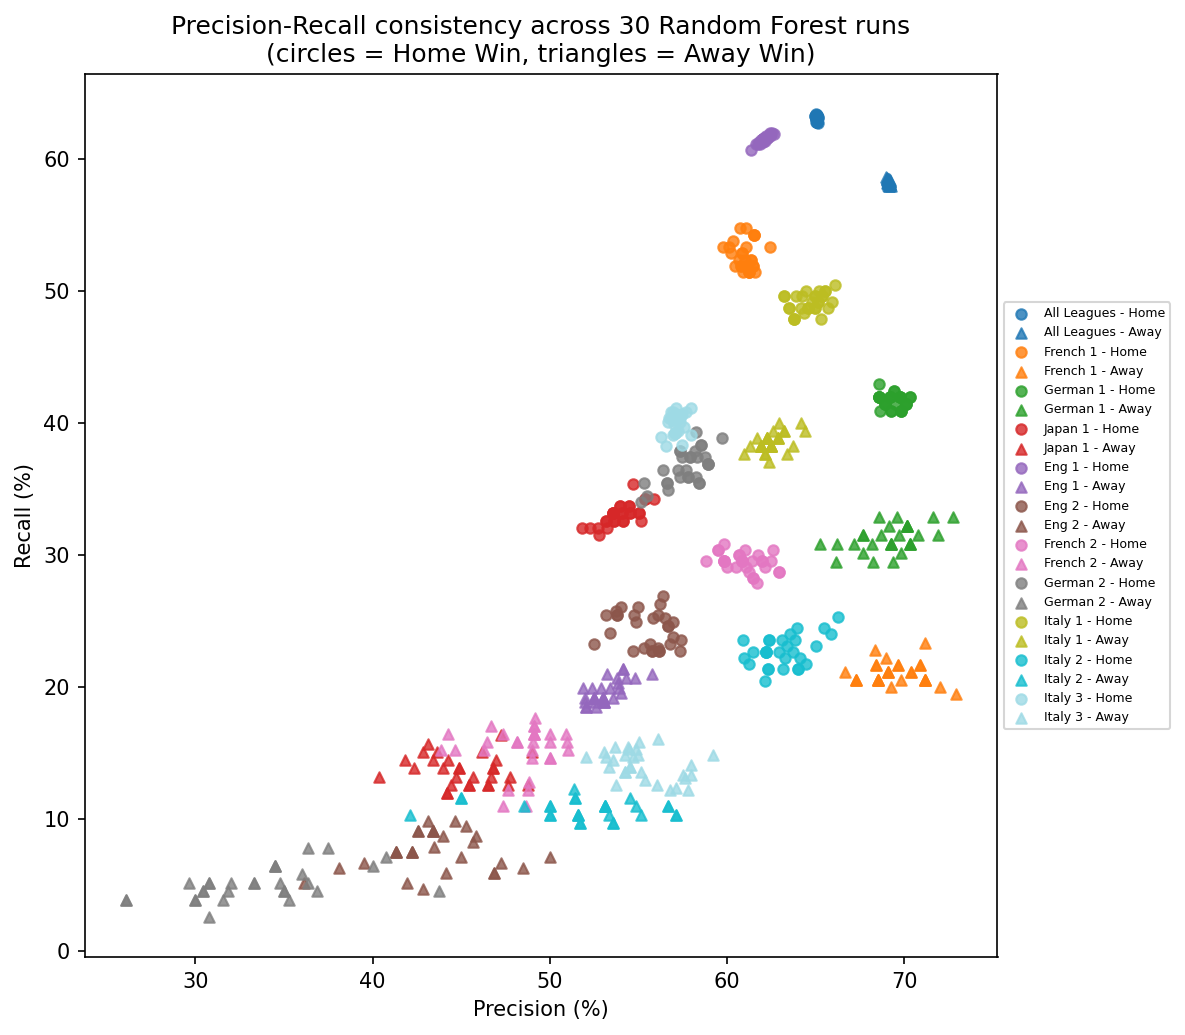
\includegraphics[scale=0.6]{all2}\caption{Precision versus Recall for each of the 30 Random Forest runs, grouped
by league and market (circles = Home Win, triangles = Away Win).\label{fig:Precision-versus-Recall}}
\end{figure}
Each cluster of points corresponds to one of the twenty-two run-groups
from Figure 1, and the tightness of a cluster is a direct visual proxy
for run-to-run consistency. The pooled-dataset clusters (blue) are
compact, confirming the low variance already observed in the box plot.
The single-league clusters, by contrast, are visibly more elongated
along the Recall axis --- most clearly for French 1 Away Win (orange
triangles), which occupies a narrow Precision band around 67--73\%
but a wide Recall band from roughly 19\% to 23\%. This pattern is
consistent with the smaller effective sample size of single-league
evaluation: Precision is estimated from a comparatively larger pool
of predicted positives, while Recall depends on the (much smaller)
count of true away-win matches actually present in that league's test
fold, making it inherently noisier from run to run. This pattern generalizes
across all ten leagues: German 2 Away Win shows the most extreme case,
with Recall collapsing to a 30-run mean of just 5.13\% despite a Precision
of 33.60\%, reflecting the very small number of true away-win matches
available within that single league's test folds.

Figure \ref{fig:Error-Rate} displays the classification error recorded
over 30 Random Forest runs for the pooled (\textquotedbl All Leagues\textquotedbl )
model in the Home Win (top) and Away Win (bottom) markets. The dashed
lines represent the corresponding mean error across all runs.

\begin{figure}[H]
\begin{centering}
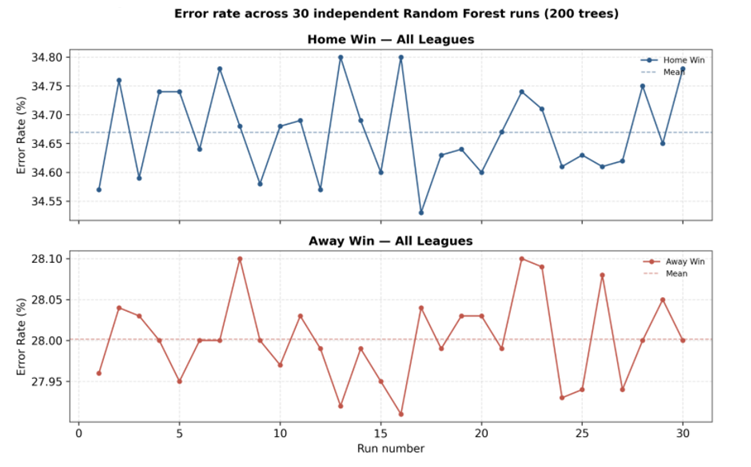
\includegraphics[scale=0.6]{football4}\caption{Error Rate (\%) of the pooled (\textquotedbl All Leagues\textquotedbl )
Random Forest model across the 30 individual runs, for the Home Win
(top) and Away Win (bottom) markets. Dashed lines mark the 30-run
mean.\label{fig:Error-Rate}}
\par\end{centering}
\end{figure}
\vspace{6pt}
No individual run departs materially from the mean trend in either
market: Home Win error oscillates within roughly 34.5--34.8\% and
Away Win error within roughly 27.9--28.1\%, with no visible upward
or downward drift across the sequence of runs. This absence of any
isolated spike or systematic trend rules out a training-order or seed-dependent
instability in the pooled configuration, and is consistent with the
narrow boxes obtained for the same group in Figure \ref{fig:Heatmap-of-Precision.}.

\begin{figure}[H]
\begin{raggedright}

\includegraphics[scale=0.4]{all}
\par\end{raggedright}
\caption{Heatmap of Precision, Recall and Error (\%) for all seven benchmarked
models on the Home Win (left) and Away Win (right) markets. The Error
column is displayed inverted (100 \textminus{} Error) so that green
consistently denotes better performance across all three columns;
the numeric labels show the original, non-inverted values.\label{fig:Heatmap-of-Precision.}}

\end{figure}
The heatmap condenses Tables of the manuscript into a single, immediately
readable panel. Random Forest and Logistic Regression stand out with
the darkest green cells in the Precision column for both markets,
confirming their role as the most structurally stable, high-precision
methods. The MLP row is the greenest in the Recall column for both
markets (63.94\% Home Win, 60.25\% Away Win), visually reinforcing
the paper's central claim that the neural network best recovers \textquotedbl hidden
value\textquotedbl{} opportunities. RBF is uniformly the weakest model,
appearing in red across nearly every cell for both markets, which
visually isolates it as the clear outlier among the seven benchmarked
algorithms.

\section{Conclusions\label{sec:Conclusions}}

This study presented a unified benchmarking and calibration framework
for football match outcome prediction, evaluating seven machine learning
paradigms --- Logistic Regression, GAM, FastTree, LightGBM, Random
Forest, RBF, and MLP --- on a large-scale dataset of approximately
230,000 matches spanning 2018--2025. Under strictly uniform experimental
conditions, Random Forest and Logistic Regression consistently delivered
the highest Precision for both the Home Win (65.11\% and 65.03\%,
respectively) and Away Win markets (69.07\% and 68.21\%, respectively),
confirming their suitability as stable, low-variance baselines. The
Multi-Layer Perceptron, in contrast, achieved the highest Recall in
both markets (63.94\% for Home Win and 60.25\% for Away Win), indicating
a superior ability to capture the non-linear feature interactions
that drive less obvious, higher-value outcomes. RBF consistently underperformed
across every metric and both markets, making it unsuitable for this
task in its present configuration.

The 30-run stability analysis conducted on the Random Forest model
reinforces these findings from a robustness perspective. When trained
and evaluated on the full, pooled multi-league dataset, the model's
Error Rate, Precision, and Recall all exhibited very low run-to-run
variance (standard deviations below 0.3 percentage points for Error),
confirming that the reported performance is a reliable structural
property of the model rather than an artifact of a favourable random
seed. However, when the same architecture was restricted to individual
leagues --- evaluated across all ten leagues available in the workbook
--- both the variance and the bias of the estimates increased substantially
and consistently, most visibly in Recall for the Away Win market,
which fell as low as 5.13\% (German 2) and did not exceed 38.55\%
(Italy 1) in any single league, compared with 58.24\% on the pooled
data. Home Win Recall showed the same directional effect, though less
severely, ranging from 22.74\% (Italy 2) to 61.49\% (Eng 1). This
pattern held across every individually evaluated league without exception
and is attributable to the reduced number of minority-class (away-win)
examples available within a single league. It carries a practical
implication for deployment: a pooled, multi-league training strategy
should be preferred over per-league retraining whenever data volume
in a target league is limited, in order to preserve both the stability
and the recall of the resulting betting signals.

Taken together, these results show that combining rigorous multi-model
benchmarking with an explicit stability analysis provides a more complete
and trustworthy picture of predictive performance than single-run
accuracy figures alone. As outlined in the Introduction, the next
phase of this research applies the Newton--Raphson de-vigging procedure
and an Isotonic Calibration layer to the raw outputs of these models,
in order to transform them into objective, well-calibrated probabilities
from which robust betting signals can be derived. While the present
study substantially extends the league-level robustness analysis to
ten individually evaluated leagues, future work will extend the present
30-run robustness protocol to the remaining six algorithms, to leagues
beyond those currently available in the workbook, and will investigate
whether league-aware feature engineering or transfer-learning strategies
can recover the Recall lost when a model is confined to a single,
smaller competition, without sacrificing the stability demonstrated
by the pooled configuration.

\vspace{6pt}


\authorcontributions{M.S. and I.G.T. conducted the experiments, employing several datasets
and provided the comparative experiments. M.S. and G.G. performed
the statistical analysis and prepared the manuscript. All authors
have read and agreed to the published version of the manuscript.}

\funding{This research has been financed by the European Union : Next Generation
EU through the Program Greece 2.0 National Recovery and Resilience
Plan , under the call RESEARCH -- CREATE -- INNOVATE, project name
“iCREW: Intelligent small craft simulator for advanced crew training
using Virtual Reality techniques\textquotedbl{} (project code:TAEDK-06195).}

\institutionalreview{Not applicable.}

\dataavailability{The original contributions presented in this study are included in
the article. Further inquiries can be directed to the corresponding
author. }

\conflictsofinterest{The authors declare no conflicts of interest.}

\appendixtitles{no}

\appendix

\begin{adjustwidth}{-\extralength}{0cm}{}


\reftitle{References}
\begin{thebibliography}{99}
\bibitem[(2006)]{physics_ml1} Raissi, M., \& Karniadakis, G. E. (2018).
Hidden physics models: Machine learning of nonlinear partial differential
equations. Journal of Computational Physics, 357, 125-141.

\bibitem{physics_ml2}Kashinath, K., Mustafa, M., Albert, A., Wu,
J. L., Jiang, C., Esmaeilzadeh, S., ... \& Prabhat, N. (2021). Physics-informed
machine learning: case studies for weather and climate modelling.
Philosophical Transactions of the Royal Society A, 379(2194), 20200093.

\bibitem[(2006)]{astronomy_ml1}Viquar, M., Basak, S., Dasgupta, A.,
Agrawal, S., \& Saha, S. (2019). Machine learning in astronomy: A
case study in quasar-star classification. Emerging Technologies in
Data Mining and Information Security: Proceedings of IEMIS 2018, Volume
3, 827-836.

\bibitem[(2006)]{astronomy_ml2}Luo, S., Leung, A. P., Hui, C. Y.,
\& Li, K. L. (2020). An investigation on the factors affecting machine
learning classifications in gamma-ray astronomy. Monthly Notices of
the Royal Astronomical Society, 492(4), 5377-5390.

\bibitem[(2006)]{chemistry_ml1}Meuwly, M. (2021). Machine learning
for chemical reactions. Chemical Reviews, 121(16), 10218-10239.

\bibitem{chemistry_ml2}J.A. Aguiar, M.L. Gong, T.Tasdizen, Crystallographic
prediction from diffraction and chemistry data for higher throughput
classification using machine learning, Computational Materials Science
\textbf{173}, 109409, 2020.

\bibitem[(2006)]{med_ml1}S.S. Yadav, S.M. Jadhav, Deep convolutional
neural network based medical image classification for disease diagnosis.
J Big Data \textbf{6}, 113, 2019.

\bibitem{med_ml2}L. Qing, W. Linhong , D. Xuehai, A Novel Neural
Network-Based Method for Medical Text Classification, Future Internet
\textbf{11}, 255, 2019. 

\bibitem[(2006)]{econ_ml1}Athey, S. (2018). The impact of machine
learning on economics. In The economics of artificial intelligence:
An agenda (pp. 507-547). University of Chicago Press.

\bibitem{econ_ml2}R. Hafezi, J. Shahrabi, E. Hadavandi, A bat-neural
network multi-agent system (BNNMAS) for stock price prediction: Case
study of DAX stock price, Applied Soft Computing \textbf{29}, pp.
196-210, 2015.

\bibitem{nn_image}Ghai, D., Tripathi, S. L., Saxena, S., Chanda,
M., \& Alazab, M. (Eds.). (2022). Machine learning algorithms for
signal and image processing. John Wiley \& Sons.

\bibitem{nn_timeseries}Ahmed, N. K., Atiya, A. F., Gayar, N. E.,
\& El-Shishiny, H. (2010). An empirical comparison of machine learning
models for time series forecasting. Econometric reviews, 29(5-6),
594-621.

\bibitem[(2009)]{nn1}Zou, J., Han, Y., \& So, S. S. (2009). Overview
of artificial neural networks. Artificial neural networks: methods
and applications, 14-22.

\bibitem[(2009)]{nn2}Abiodun, O. I., Jantan, A., Omolara, A. E.,
Dada, K. V., Mohamed, N. A., \& Arshad, H. (2018). State-of-the-art
in artificial neural network applications: A survey. Heliyon, 4(11).

\bibitem[(2009)]{dt1}De Ville, B. (2013). Decision trees. Wiley Interdisciplinary
Reviews: Computational Statistics, 5(6), 448-455.

\bibitem[(2009)]{dt2}Kotsiantis, S. B. (2013). Decision trees: a
recent overview. Artificial Intelligence Review, 39(4), 261-283.

\bibitem[(2009)]{svm1}Pisner, D. A., \& Schnyer, D. M. (2020). Support
vector machine. In Machine learning (pp. 101-121). Academic Press.

\bibitem[(2009)]{svm2}Valkenborg, D., Rousseau, A. J., Geubbelmans,
M., \& Burzykowski, T. (2023). Support vector machines. American journal
of orthodontics and dentofacial orthopedics, 164(5), 754-757.

\bibitem{power}Clarke, S. (2016). A review of methods for deriving
probability estimates from betting odds.

\bibitem{gam}Wood, S. N. (2017). Generalized Additive Models: An
Introduction with R (2nd ed.). Chapman and Hall/CRC.

\bibitem[(2017)]{fasttree}Price, M. N., Dehal, P. S., \& Arkin, A.
P. (2010). FastTree 2--approximately maximum-likelihood trees for
large alignments. PloS one, 5(3), e9490.

\bibitem[(2017)]{lightgbm}Ke, G., Meng, Q., Finley, T., Wang, T.,
Chen, W., Ma, W., ... \& Liu, T. Y. (2017). Lightgbm: A highly efficient
gradient boosting decision tree. Advances in neural information processing
systems, 30.

\bibitem{randomForest}Liaw, A., \& Wiener, M. (2002). Classification
and regression by randomForest. R News, 2(3), 18-22.s

\bibitem[(2009)]{elo_football}Hvattum, L. M., \& Arntzen, H. (2010).
Using ELO ratings for match result prediction in association football.
International Journal of forecasting, 26(3), 460-470.

\bibitem[(2009)]{ml_bayesian}Marcot, B. G., \& Penman, T. D. (2019).
Advances in Bayesian network modelling: Integration of modelling technologies.
Environmental modelling \& software, 111, 386-393.

\bibitem[(2009)]{bayesian_football}Owramipur, F., Eskandarian, P.,
\& Mozneb, F. S. (2013). Football result prediction with Bayesian
network in Spanish League-Barcelona team. International Journal of
Computer Theory and Engineering, 5(5), 812.

\bibitem[(2009)]{ml_logistic}Stoltzfus, J. C. (2011). Logistic regression:
a brief primer. Academic emergency medicine, 18(10), 1099-1104.

\bibitem[(2009)]{logistic_football}D. Prasetio and D. Harlili, \textquotedbl Predicting
football match results with logistic regression,\textquotedbl{} 2016
International Conference On Advanced Informatics: Concepts, Theory
And Application (ICAICTA), Penang, Malaysia, 2016, pp. 1-5, doi: 10.1109/ICAICTA.2016.7803111.

\bibitem[(2009)]{polynomial_football}Martins, R. G., Martins, A.
S., Neves, L. A., Lima, L. V., Flores, E. L., \& do Nascimento, M.
Z. (2017). Exploring polynomial classifier to predict match results
in football championships. Expert Systems with Applications, 83, 79-93.

\bibitem[(2009)]{rf_football}Schauberger, G., \& Groll, A. (2018).
Predicting matches in international football tournaments with random
forests. Statistical Modelling, 18(5-6), 460-482.

\bibitem[(2009)]{attr_football}Danisik, N., Lacko, P., \& Farkas,
M. (2018, August). Football match prediction using players attributes.
In 2018 World symposium on digital intelligence for systems and machines
(DISA) (pp. 201-206). IEEE.

\bibitem[(2009)]{dolores_football}Constantinou, A. C. (2019). Dolores:
a model that predicts football match outcomes from all over the world.
Machine learning, 108(1), 49-75.

\bibitem[(2009)]{ml_boosting}Natekin, A., \& Knoll, A. (2013). Gradient
boosting machines, a tutorial. Frontiers in neurorobotics, 7, 63623.

\bibitem[(2009)]{boost_football}Baboota, R., \& Kaur, H. (2019).
Predictive analysis and modelling football results using machine learning
approach for English Premier League. International Journal of Forecasting,
35(2), 741-755.

\bibitem[(2009)]{deep_football}Rahman, M. A. (2020). A deep learning
framework for football match prediction. SN Applied Sciences, 2(2),
165.

\bibitem{ml.net}Microsoft. (2026). ML.NET: Machine Learning for .NET.
Retrieved June 30, 2026, from \url{https://dotnet.microsoft.com/en-us/apps/machinelearning-ai/ml-dotnet}

\bibitem[(1989)]{lbfgs}Liu, D. C., \& Nocedal, J. (1989). On the
limited memory BFGS method for large scale optimization. Mathematical
programming, 45(1), 503-528.

\bibitem[(1991)]{rbf1}J. Park and I. W. Sandberg, Universal Approximation
Using Radial-Basis-Function Networks, Neural Computation \textbf{3},
pp. 246-257, 1991.

\bibitem{rbf2}G.A. Montazer, D. Giveki, M. Karami, H. Rastegar, Radial
basis function neural networks: A review. Comput. Rev. J \textbf{1},
pp. 52-74, 2018.

\end{thebibliography}
%%%%%%%%%%%%%%%%%%%%%%%%%%%%%%%%%%%%%%%%%%
%% for journal Sci
%\reviewreports{\\
%Reviewer 1 comments and authors' response\\
%Reviewer 2 comments and authors' response\\
%Reviewer 3 comments and authors' response
%}
%%%%%%%%%%%%%%%%%%%%%%%%%%%%%%%%%%%%%%%%%%

\PublishersNote{}

\end{adjustwidth}{}
\end{document}
